\chapter{Related Work}
\label{chap:relatedwork}
\numberwithin{equation}{chapter}
Creating a generic configurable search engine that includes a simple user interface will require research on how the current search engine works and what are the existing commercial or open-source solutions that offer a similar feature that allows the search engine to be configured via user interface reactions. This chapter will explain an overview of the Google search engine architecture since the basic architecture concepts will be reused with some modifications in this thesis. Then a list of the existing solutions used to crawl the web will be discussed.  



\section{High Level Google Architecture}

The Google search engine's design gives a good overview of the essential components to create a scalable search engine. Hence, it is a great starting point for any search engine research; we will explain it in this section. Most code written in the Google search engine was implemented in C or C++ for efficiency and because it can run on either Solaris or Linux [2]. Google uses distributed crawlers to download internet web pages. The URLserver keeps a list of the available found URLs that need to be crawled by the crawlers. URLserver acts as a load balancer that sends the URLs to the following free crawler. Afterwards, the crawlers download the documents needed from the page, associate a unique ID for this page called docID, and then the page's content are stored in Soreservers. Storeservers then compress the pages and save them on a repository. The indexer component then uncompresses the pages and parses them. Each document is then converted into a set of words called hits. The hits represent the word and its position in the document. Afterwards, the indexer distributes those hits into barrels. Moreover, the indexer collects links found in the crawled page and stores them in the anchor's file. The anchors' file contains the links and their relationship with each other [2].


\begin{figure}[h]	
     \centering
     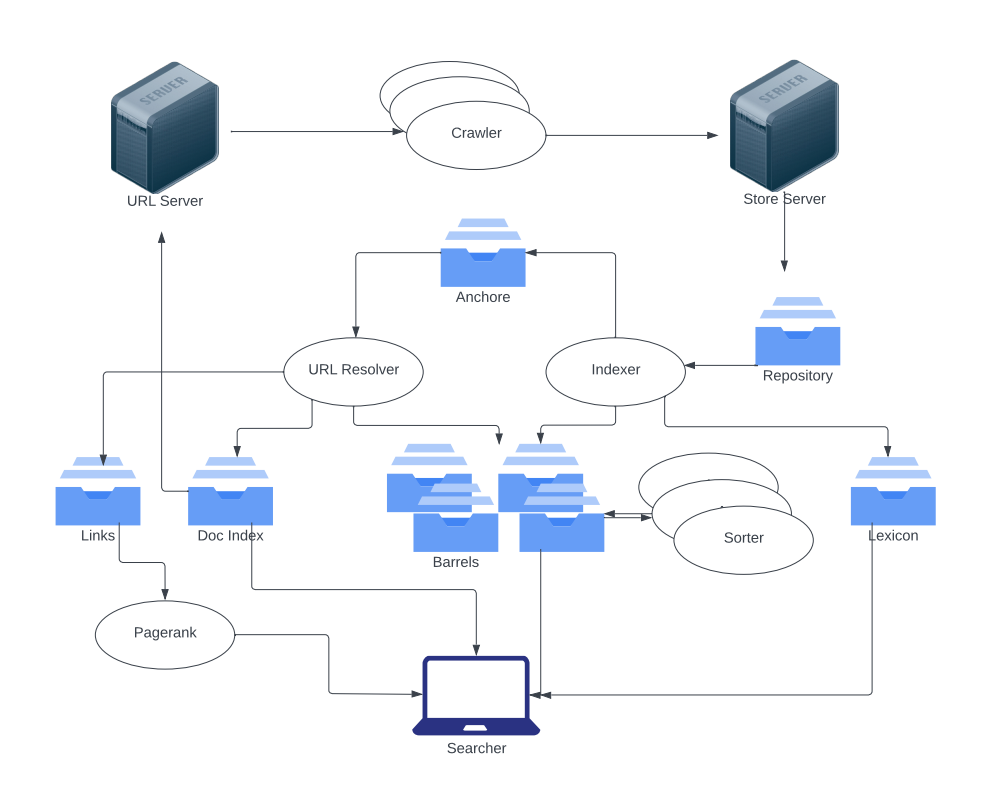
\includegraphics[width=10cm]{images/google_arch.png}
     \caption{High level view of Google web crawlers archeticture.}
     \label{fig:google-arch}
\end{figure}

The URLresolver reads the links from the anchors' file and converts the relative URLs into absolute URLs. The URLs are then assigned to their docID. The links database saves pairs of docIDs that will be used to compute PageRanks for all the documents. 

Initially organized by docID, the barrels are then rearranged by the sorter based on wordID. This process generates an inverted index. Moreover, the sorter generates a list of wordIDs and corresponding offsets within the inverted index. 

\section{Web Crawlers}
The concept of web crawling dates back to the early 1990s when the World Wide Web was still in its infancy.

WebCrawler, created by Brian Pinkerton in 1994, is considered the first true web crawler-powered search engine. While some may claim that title for Wandex is due to its potential, it was never designed to be used in this way. Wandex lacked some critical features to make it a general-purpose search engine.

One of the major innovations of WebCrawler was its full-text searchability. This ability made it popular and highly functional. It continues to operate as a search engine, although not as popular as Google, Yahoo, Bing, Yandex, or Baidu.

Modern web crawlers face many challenges and complexities, such as dynamic content, user interaction, authentication, robots.txt files, and ethical issues. Some examples of modern web crawlers are Googlebot, Bingbot, and Internet Archive

Web crawlers have evolved during the last few decades, with different designs and implementations to crawl and index the internet. Below is an enumeration of some of the architectural designs utilized in the development of all-encompassing web crawlers [3]:


\begin{itemize}
  \item \textbf{RBSE [Eic94]} Considered as one of the first Web crawlers to be published. Made of two components: the first component,
“spider”, uses a queue in a database. The second component, “mite”, is a modified browser that downloads the pages from the Web.
  \item \textbf{WebCrawler [Pin94]}  The initial publicly accessible full-text index of a specific portion of the World Wide Web was established. The approach involved leveraging lib-WWW for page downloads and employing an additional tool to parse and arrange URLs, ensuring a breadth-first approach to navigating the web graph.
  \item \textbf{World Wide Web Worm [McB94]} was a crawler designed to construct a basic index comprising document titles and corresponding URLs. This index could be queried by utilising the grep command in the UNIX operating system.
  \item \textbf{Google Crawler [BP98]} Google has been the market's dominant search engine for the last few decades. In March 2023, Google’s global market share was 85.53% [4].
The crawler was integrated with the indexing, and since this thesis has some similarity with the Google search engine design, we will explain this in-depth in the ext subsection [Google architecture]
  \item \textbf{Ubicrawler [BCSV04]} Is a Java-based distributed crawler with no central process and several identical “agents”. The crawler is implemented to provide high scalability and be tolerant of failures.
\end{itemize}

Although the previously mentioned crawlers offer a wide range of features and are great to be used as generic crawlers to fetch all web pages, they need to provide a simple user interface to configure them based on user needs. This is what this thesis tries to tackle and investigate. 

Nowadays, data scientist uses different tools to crawl and parse internet content. Each tool has its pros and cons and serves a different use case than the other. The following list goes through some of the most well know crawlers and explains how the proposed solution in this thesis differs.  


\begin{itemize}
  \item \textbf{Beautiful Soup:} Beautiful Soup is an open-source library that stands out as a widely used web scraping library that simplifies retrieving data from HTML and XML documents. Beautiful Soup demonstrates exceptional proficiency in parsing HTML documents, streamlining the task of retrieving particular components like headings, paragraphs, tables, and links. Beautiful Soup is not a search engine. It lacks the most fundamental search engine components; hence, it requires programming skills and can only be used to implement a search engine. Beautiful Soup can only parse the first seen page HTML version. Meaning it does not include the Javascript code. This is bad as most modern web pages use Javascript heavily to improve the page's latency. For example, pagination will be an issue for Beautiful Soup.

  \item \textbf{Scrapy:} It is an open-source, powerful and flexible tool that easily crawls and parses different websites. It allows the creation of custom spiders to crawl multiple pages. Easy to scale makes it suitable for large projects. This tool is perfect for programmers but not for non-technical users, as it requires good knowledge of Python programming.

  \item \textbf{Selenium:} It is an open-source, robust and adaptable solution for web scraping, enabling the automation of browser actions, interaction with web pages, and data extraction from online sources. It shares some features with the Beautiful Soupe as it is an excellent tool for parsing the HTML DOM. Still, it also overcomes the issue previously mentioned about rendering Javascript and supporting dynamic contents as paginations. Interactive browser automation makes it easy to mimic the user's behaviour which makes it easier to navigate towards hidden content that requires events and human interactions. Selenium alone can be used as a search engine; however, it will be used in this thesis as a fundamental tool for the search engine implemented.    

  \item \textbf{ParseHub:} A web crawler tool with a friendly User Interface requiring no programming skills. It is one of the top choices of most data scientists. The massive advantage of ParseHub is the point-and-click interface provided. It makes data extraction extremely easy. ParseHub offers both free and paid plans. The free plan allows users to scrape up to 200 pages per run, which, as we will see, is too slow for a crawler. Moreover, it is not possible to configure the crawling algorithms with this tool, and the indexing component does not exist. Since this tool is the most similar tool to the solution implemented by this thesis, it will be used as a comparison in the evaluation chapter. 
\end{itemize}
